\begin{figure*}
%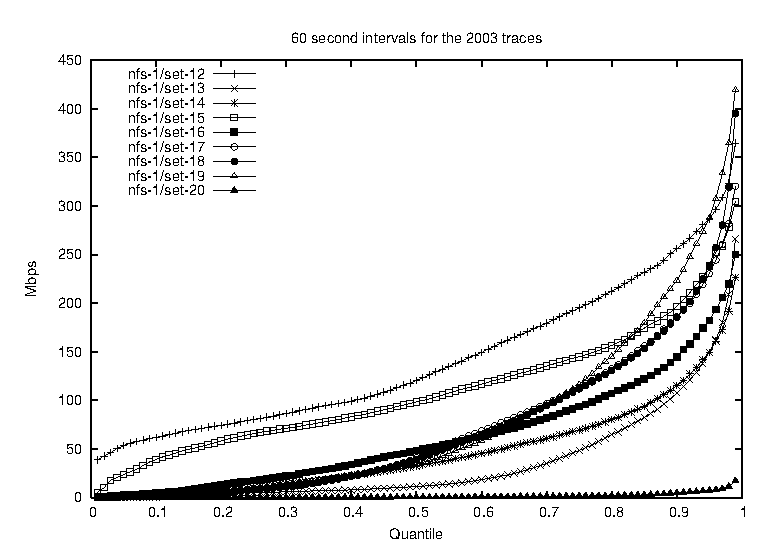
\epsfig{width=2.1in, angle=0, file=graphs/Mbps-nfs-1.ps}
%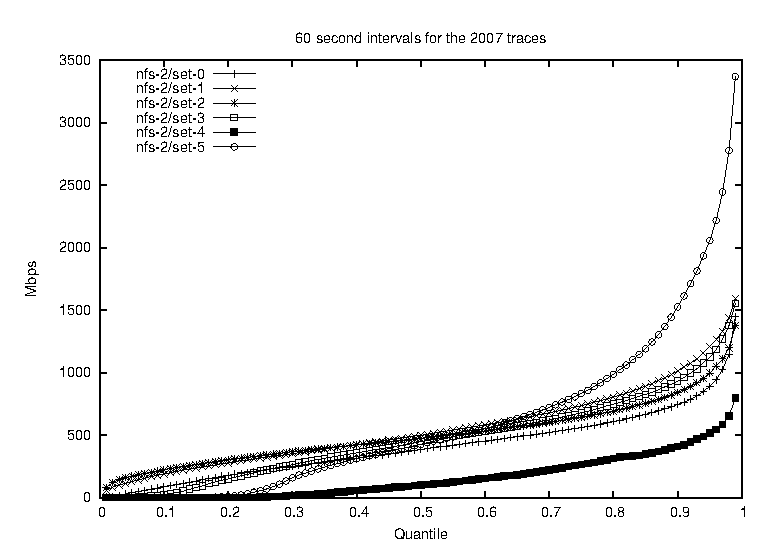
\epsfig{width=3.2in, angle=0, file=graphs/Mbps-nfs-2.ps}
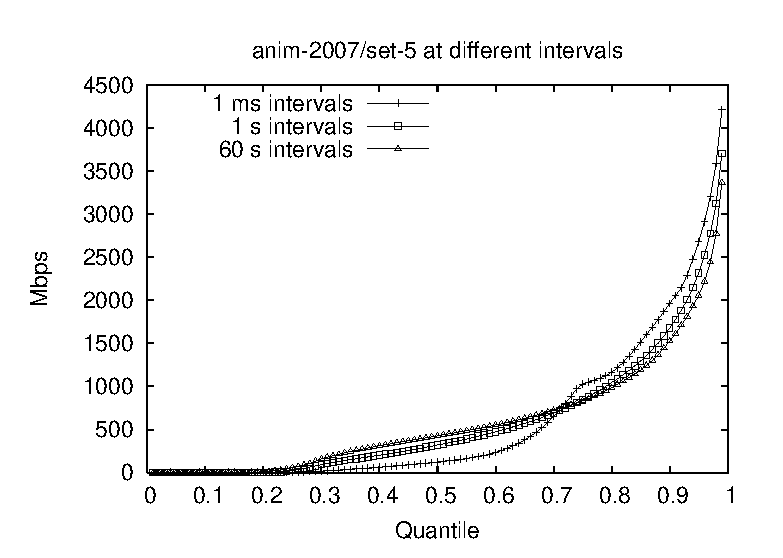
\epsfig{width=3.3in, angle=0, file=graphs/Mbps-nfs-2-set-5.ps}
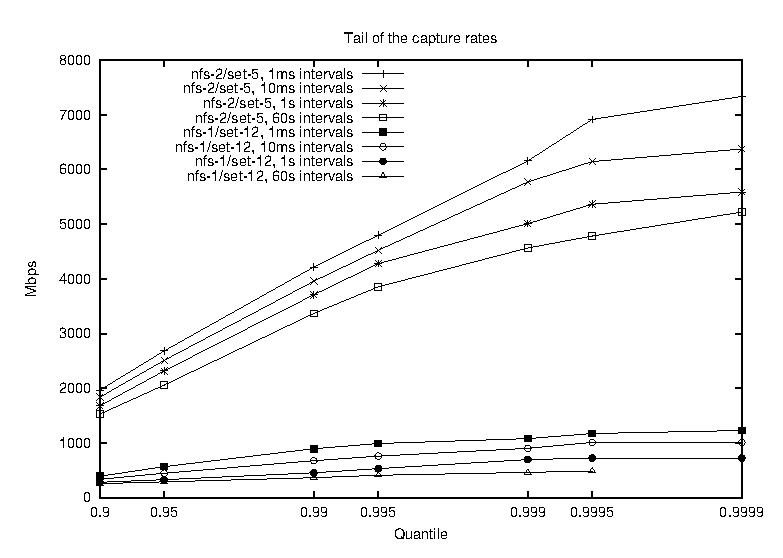
\epsfig{width=3.3in, angle=0, file=graphs/Mbps-tails.ps}
\vspace{-0.2in}
\caption{Bandwidth measured in the collection process.  In Figure (b),
anim-2007/set-5 at different intervals is the top group of 4 lines, and
anim-2003/set-12 is the bottom group of 4 lines. With 60s intervals, 
anim-2003/set-12 does not show the 0.9999 quantile 
because there were insufficient data points.}
\label{fig:bwrolling-mbps}
\end{figure*}


% LocalWords:  anim mbps
